\documentclass[aps,10pt,onecolumn,prx,superscriptaddress,longbibliography,nofootinbib]{revtex4-2}

\usepackage[T1]{fontenc}
\usepackage{lmodern}
\usepackage{amsmath,amssymb,amsthm,mathtools}
\usepackage{array}[=2016-10-06]
\usepackage{booktabs}
\usepackage{graphicx}
\usepackage{microtype}
\usepackage{xcolor}
\usepackage{tcolorbox}
\usepackage{tikz}
\usetikzlibrary{arrows.meta,positioning,calc}
\usepackage[colorlinks=true,citecolor=black,linkcolor=black,urlcolor=black]{hyperref}
\setcitestyle{super,sort&compress}
\setlength{\emergencystretch}{2em}
\graphicspath{{figures/}{../outputs/figures/}}

\newtcolorbox{protocolbox}[2][]{
    float=htbp,
    colback=gray!5!white,
    colframe=black!55!white,
    fonttitle=\bfseries,
    coltitle=black,
    title=#2,
    sharp corners,
    boxsep=5pt,
    left=5pt,
    right=5pt,
    top=5pt,
    bottom=5pt,
    #1
}

\newcommand{\ket}[1]{\lvert #1\rangle}
\newcommand{\bra}[1]{\langle #1\rvert}
\newcommand{\Tr}{\operatorname{Tr}}
\newcommand{\id}{\mathbb I}
\newcommand{\hbin}{h_2}
\newcommand{\EC}{\ell_{\mathrm{EC}}}
\newcommand{\perpout}{\perp}
\newcommand{\rPCHSH}{\mathrm{rPCHSH}}
\newcommand{\rPhase}{\mathrm{rPhase}}
\newcommand{\rHybrid}{\mathrm{rHybrid}}
\newtheorem{theorem}{Theorem}
\newtheorem{proposition}[theorem]{Proposition}
\newtheorem{lemma}[theorem]{Lemma}
\newtheorem{corollary}[theorem]{Corollary}
\newtheorem{definition}[theorem]{Definition}
\newtheorem{remark}[theorem]{Remark}

\newcommand{\resultfigure}[2]{\includegraphics[width=#2\linewidth]{#1}}

\hypersetup{
  pdftitle={Device-Independent Conference Key Agreement via Tripartite Routed Bell Tests},
  pdfauthor={Xin Kuang, Xingyuan Bu, Yuqian Zhou, Yi-Zheng Zhen, Yunguang Han}
}

\begin{document}

\title{Device-Independent Conference Key Agreement via Tripartite Routed Bell Tests}
\author{Xin Kuang}
\affiliation{College of Computer Science and Technology, Nanjing University of Aeronautics and Astronautics, Nanjing 211106, China}
\author{Xingyuan Bu}
\affiliation{College of Computer Science and Technology, Nanjing University of Aeronautics and Astronautics, Nanjing 211106, China}
\author{Yuqian Zhou}
\affiliation{College of Computer Science and Technology, Nanjing University of Aeronautics and Astronautics, Nanjing 211106, China}
\author{Yi-Zheng Zhen}
\affiliation{Hefei National Research Center for Physical Sciences at the Microscale and School of Physical Sciences, University of Science and Technology of China, Hefei 230026, China}
\affiliation{Shanghai Research Center for Quantum Science and CAS Center for Excellence in Quantum Information and Quantum Physics, University of Science and Technology of China, Shanghai 201315, China}
\author{Yunguang Han}
\email{hanyunguang@nuaa.edu.cn}
\affiliation{College of Computer Science and Technology, Nanjing University of Aeronautics and Astronautics, Nanjing 211106, China}

\begin{abstract}
Can nearby Bell tests certify a conference key when the complete distant observations alone cannot guarantee one? We study a tripartite routed experiment in which Bob and Charlie must recover Alice's key from separate records. For the ideal GHZ target, joint phase information is available when both travelling systems arrive, whereas reconciliation is limited by the weaker receiver. A matching erasure attack yields the exact rate of the phase and hybrid protocols, with a symmetric remote-efficiency threshold of approximately $61.8\%$. With source noise and imperfect nearby detection, an explicit attack reproduces the complete distant hybrid behavior, which is itself Bell-nonlocal, and prevents positive key using messages from Alice alone. Adding nearby observations certifies positive key at the same target. We compare three remote measurement choices, retain nondetections as a third receiver outcome, and identify the joint correlations needed to exclude a dephased realization. The analysis assumes asymptotic collective attacks and fixed raw-key records.
\end{abstract}

\maketitle

\section{Introduction}\label{sec:introduction}

A conference key must be secret from an eavesdropper and recoverable by every legitimate user. Device-independent conference key agreement (DICKA) infers that security from observed correlations, without characterizing the source or measurement devices~\cite{Brunner2014,Ribeiro2018,Holz2020,Murta2020}. It extends device-independent quantum key distribution (DIQKD) to a shared task across a network~\cite{Ekert1991,Acin2007,Primaatmaja2023,Epping2017}. Under transmission loss, the joint observations available to test secrecy can differ substantially from the records available to an individual receiver. This distinction is important when the links have unequal efficiencies.

Loss weakens the correlations available for loophole-free certification, often imposing demanding efficiency requirements on distant detectors~\cite{ClauserHorne1974,MassarPironio2003}. Multipartite Bell inequalities and distribution schemes address different aspects of this problem~\cite{Holz2020,Grasselli2023,Ishihara2025,Azuma2023}. Routed Bell tests instead use high-quality measurements near the source to constrain correlations observed after long-distance transmission~\cite{Chaturvedi2024,Lobo2024}. In randomly selected rounds, the travelling systems are directed to nearby test stations. Since the source and Alice's measurements cannot adapt to the route, the two branches must admit a common explanation.

The short-range quantum (SRQ) benchmark introduced by Lobo, Pauwels and Pironio~\cite{Lobo2024} distinguishes quantum transmission from quantum processing near the source followed by classical communication~\cite{Masini2024}. For key distribution, local Bell calibration and its entropy-based security analysis are already established~\cite{Lim2013,TanWolf2024}. Bipartite routed protocols using CHSH, complementary-basis or combined measurements improve loss tolerance when the nearby tests are sufficiently good, but remain sensitive to imperfections in those tests~\cite{LeRoy2025}.

Extending this picture to conference key agreement requires accounting for both joint quantum observations and separate decoding tasks. In a tripartite protocol, phase information relevant to secrecy may require both travelling systems to arrive, while Bob and Charlie must each recover Alice's key from their own records. Grouping the receivers into one effective party obscures this distinction. Moreover, Eve can attack the two arms jointly, and simulating either required receiver can compromise the common key. The question is therefore how short-path certification constrains the security of this shared task: can it certify a positive conference-key rate when the complete long-path observations alone cannot guarantee one?

We answer this question for a common-switch GHZ protocol. Nearby calibration and remote phase information give an exact ideal rate, with a matching attack that bounds even stochastic or blockwise preprocessing by Alice. For a noisy hybrid experiment, an attack reproduces every distant probability, yet nearby observations at the same target certify a positive rate. The distant behavior is already Bell-nonlocal, so routing supplies a security constraint beyond the exclusion of classical remote explanations. Three choices of remote tests reveal the roles of parity and direct phase information; a controlled removal of correlations shows why nearby calibration and key agreement cannot replace the latter. All converse statements concern the fixed raw records and key-distillation messages sent only by Alice.

\section{Tripartite Routed Conference Key Agreement}\label{sec:framework}

\subsection{Routed architecture}

In a bipartite routed Bell experiment, a switch directs one travelling system either to a nearby test station or to a distant receiver~\cite{Chaturvedi2024,Lobo2024}. The source and Alice's measurements cannot adapt to this choice. High-quality nearby observations therefore constrain the same quantum realization that must explain the lossy distant experiment~\cite{TanWolf2024,LeRoy2025}.

Our tripartite architecture is shown in Fig.~\ref{fig:architecture}. Alice measures one subsystem at a fixed station, while a common switch \(r\in\{S,L\}\) directs the other two to either the nearby stations \((B_S,C_S)\) or the distant stations \((B_L,C_L)\). We denote the routed behavior by \(\mathbf P=(P_S,P_L)\), with conditional probabilities \(P_r(a,b,c|x,y,z)\). The route is sampled independently of the source and the devices' initial state, and remains unavailable to the source and Alice until Alice produces her output. Eve may attack the two travelling systems jointly. Bob and Charlie must nevertheless decode the common key separately, from records that can have different losses.

Alice has measurements \(A_0,A_1\), Bob has measurements \(B_y^r\), and Charlie has measurements \(C_z^r\). In the honest GHZ implementation, \(A_0,B_2^L,C_1^L\) measure \(Z\), while \(A_1,B_3^L,C_0^L\) measure \(X\). The key inputs \((x,y,z)=(0,2,1)\) therefore select \(ZZZ\), and the direct phase inputs \((1,3,0)\) select \(XXX\). Bob's inputs \(y=0,1\) use rotated \(Z/X\) bases for the parity test. These directions specify the honest reference only; the numbered inputs remain uncharacterized in the security analysis.

\begin{figure}[htbp]
\centering
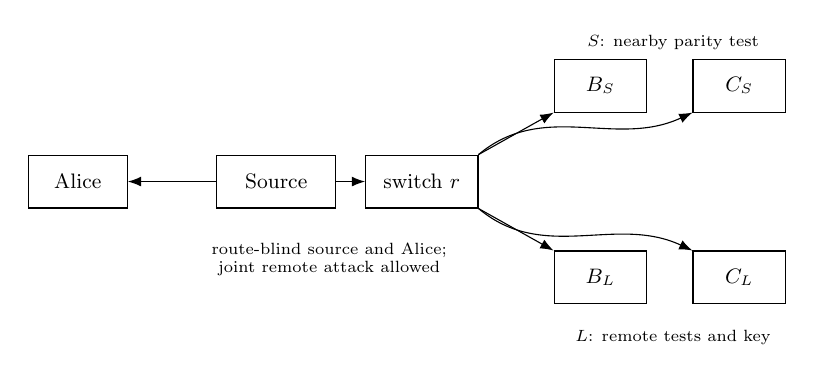
\begin{tikzpicture}[>=Latex,scale=.84,every node/.style={transform shape},font=\small]
  \node[draw,minimum height=8mm,minimum width=18mm] (Q) at (0,0) {Source};
  \node[draw,minimum height=8mm,minimum width=15mm] (A) at (-3.0,0) {Alice};
  \node[draw,minimum height=8mm,minimum width=17mm] (sw) at (2.2,0) {switch \(r\)};
  \node[draw,minimum height=8mm,minimum width=14mm] (BS) at (4.9,1.45) {\(B_S\)};
  \node[draw,minimum height=8mm,minimum width=14mm] (CS) at (7.0,1.45) {\(C_S\)};
  \node[draw,minimum height=8mm,minimum width=14mm] (BL) at (4.9,-1.45) {\(B_L\)};
  \node[draw,minimum height=8mm,minimum width=14mm] (CL) at (7.0,-1.45) {\(C_L\)};
  \draw[->] (Q)--(A);
  \draw[->] (Q)--(sw);
  \draw[->] (sw.north east)--(BS.south west);
  \draw[->] (sw.north east) to[out=40,in=205] (CS.south west);
  \draw[->] (sw.south east)--(BL.north west);
  \draw[->] (sw.south east) to[out=-40,in=155] (CL.north west);
  \node[font=\scriptsize] at (6,2.1) {\(S\): nearby parity test};
  \node[font=\scriptsize] at (6,-2.35) {\(L\): remote tests and key};
  \node[font=\scriptsize,align=center] at (.8,-1.18) {route-blind source and Alice;\\joint remote attack allowed};
\end{tikzpicture}
\caption{A common switch directs both travelling systems to nearby or remote stations. All measurement devices are uncharacterized. The source and Alice remain independent of the route until Alice records her output.}
\label{fig:architecture}
\end{figure}

\subsection{Conference-key protocol}\label{sec:conference-protocol}

The parties operate isolated, uncharacterized devices and communicate over an authenticated public channel. Alice and the nearby stations record \(\{+1,-1\}\), assigning nondetections through \(\perpout\mapsto+1\). Both remote stations retain \(\{+1,-1,\perpout\}\) in every test and key input, so erasure flags remain available for testing and decoding~\cite{LeRoy2025}. The reference calculations use \(\eta_A=1\), \(\eta_{B_S}=\eta_{C_S}=\eta_S\), and distant efficiencies \(\eta_B,\eta_C\); these generate target data rather than trusted restrictions on the devices. Every long-route key round is retained, including nondetections. Rates are per attempted key round; throughput per source use also includes route and setting probabilities.

The variants in Table~\ref{tab:protocol-family} share the nearby test and \(ZZZ\) key context. The parity protocol, \(\rPCHSH\), uses the rotated parity-test bases; \(\rPhase\) uses the direct \(XXX\) phase correlation; \(\rHybrid\) includes both. Secrecy need not be certified by violation of one common remote Bell expression. Section~\ref{sec:protocols} specifies the honest measurement directions.

\begin{table}[t]
\caption{Protocol variants with Alice's inputs $x=0,1$, the same nearby parity test, ternary remote outputs and key inputs $(0,2,1)$.}
\label{tab:protocol-family}
\begin{ruledtabular}
\begin{tabular}{lccc}
Protocol & Bob's remote inputs & Charlie's remote inputs & Role of remote tests\\
\hline
\(\rPCHSH\) & $0,1,2$ & $0,1$ & tilted parity-CHSH data\\
\(\rPhase\) & $2,3$ & $0,1$ & direct phase correlations\\
\(\rHybrid\) & $0,1,2,3$ & $0,1$ & both tests
\end{tabular}
\end{ruledtabular}
\end{table}

\begin{protocolbox}{Unified Routed Tripartite DICKA Protocol}
\label{prot:routed}

\textbf{Inputs and devices.}
The parties use the stations in Fig.~\ref{fig:architecture}, trusted private randomness for routes, settings and test samples, and an authenticated public channel.

\begin{enumerate}
\item \textbf{For every round \(i\in[n]\):}
\begin{enumerate}
  \item \textit{Distribution.}
  An untrusted source distributes one system to Alice and two travelling systems to the common switch.

  \item \textit{Routing.}
  A fresh variable \(r_i\in\{S,L\}\) is sampled independently of the source and its initial state, with \(\Pr[r_i=S]=\mu\), and supplied to the isolated switch. Its value is causally unavailable to the source and Alice's device until Alice has recorded her output. If \(r_i=S\), the travelling systems are sent to \(B_S,C_S\); if \(r_i=L\), they are sent to \(B_L,C_L\).

  \item \textit{Setting choice.}
  Alice chooses $x_i\in\{0,1\}$ independently of $r_i$. On the nearby branch, Bob chooses $y_i\in\{0,1\}$ and Charlie uses $z_i=0$, producing the parity-CHSH calibration data. On the remote branch, Bob and Charlie choose inputs from the protocol-dependent sets in Table~\ref{tab:protocol-family}. The context $(x_i,y_i,z_i)=(0,2,1)$ is the candidate key context; all other remote contexts are test contexts.

  \item \textit{Measurement and recording.}
  The selected settings are supplied before the devices produce outputs. The parties record \(A'_i,B'_i,C'_i\) using the conventions above, for every test and key input. They announce $r_i,x_i,y_i,z_i$ only after the outputs have been fixed.
\end{enumerate}

\item \textbf{Parameter estimation and key distillation:}
\begin{enumerate}
  \item \textit{Parameter estimation.}
  The parties announce the routes and settings, reveal all nearby rounds, all remote test contexts and a random sample of the remote key rounds, and estimate the declared coordinates of \(\mathbf P=(P_S,P_L)\). They abort unless the resulting confidence region satisfies the predetermined acceptance and positive-rate conditions. In the asymptotic analysis below, sampling fluctuations vanish and the retained behavior is treated as known.

  \item \textit{Raw records.}
  The unrevealed long-route rounds at inputs $(0,2,1)$ form Alice's binary raw string. Bob and Charlie retain the corresponding ternary records as separate decoding information.

  \item \textit{Error correction and privacy amplification.}
  Alice may preprocess her raw string and broadcasts error-correction information for each receiver to decode from their own record, followed by a privacy-amplification seed. During key distillation, only Alice sends public messages: Bob and Charlie do not provide feedback or select key rounds according to their detection records. All three parties then produce the conference key or abort.
\end{enumerate}
\end{enumerate}
\end{protocolbox}

We analyze asymptotic i.i.d. behavior under collective attacks. Eve may purify the source, attack both remote systems jointly and postpone her measurement until after public communication. The restriction to messages from Alice concerns key distillation after parameter estimation, not the parties' earlier disclosure of routes, settings and test data.

\subsection{Short-range quantum correlations}

A nearby Bell violation alone does not establish quantum transmission to either distant station. Eve could measure the travelling systems near the source and send only classical instructions to Bob and Charlie. Such an explanation still permits quantum nearby correlations. The SRQ model makes this alternative precise~\cite{Lobo2024}.

\begin{definition}[Tripartite SRQ behavior]\label{def:srq}
A routed behavior is SRQ-compatible if a single pre-route state \(\rho_{ABC}\), route-blind Alice measurements, nearby measurements, and a parent POVM \(\{N_\omega\}\) on the two travelling systems reproduce both branches as
\begin{align}
 P_S(a,b,c|x,y,z)&=\Tr[(A_{a|x}\otimes B^S_{b|y}\otimes C^S_{c|z})\rho_{ABC}],\label{eq:srq-short}\\
 P_L(a,b,c|x,y,z)&=\sum_\omega\Tr[(A_{a|x}\otimes N_\omega)\rho_{ABC}]
 p_B(b|y,\omega)p_C(c|z,\omega).
 \label{eq:srq-long}
\end{align}
The remote response alphabets are \(b,c\in\{+1,-1,\perpout\}\).
\end{definition}

The joint parent measurement \(N_\omega\) is independent of the remote inputs \(y,z\). It can therefore be performed before those inputs are chosen, with its classical outcome sent to both remote stations. Quantum processing remains near the source; only classical information needs to travel to the receivers. Crucially, a local model of \(P_L\) alone is not enough: the same state and Alice measurements must also reproduce \(P_S\).

This model has a direct cryptographic consequence. Eve can keep the parent outcome and draw a synthetic key record with the same conditional distribution as either receiver's record. She can then apply that receiver's decoder to Alice's public messages. Because every participant must recover the conference key, simulating one required receiver suffices.

\begin{proposition}[SRQ obstruction to conference-key certification]\label{prop:srq-obstruction}
An SRQ-compatible routed behavior cannot guarantee a positive asymptotic conference-key rate with the fixed key inputs \((0,2,1)\) and post-processing messages sent only by Alice, including stochastic or blockwise preprocessing by Alice.
\end{proposition}

Appendix~\ref{app:srq} proves this statement, including the disclosed test records. Excluding SRQ is thus necessary for key certification in this protocol class, but is not sufficient: quantum attacks outside SRQ can also prevent a key. We will encounter such an attack for a Bell-nonlocal remote behavior in Sec.~\ref{sec:routing-secrecy}. Analytical SRQ witnesses are retained in Appendix~\ref{app:srq} as diagnostics; their violation is not a required step in the entropy analysis.

\section{Analytical Security and Ideal Rates}\label{sec:protocols}

\subsection{Honest reference model}

The protocol specifies which data are observed, not the source or measurements that untrusted devices must implement. To evaluate loss tolerance, we use the following GHZ reference model. Assigning the signed values $(+1,-1,0)$ to the remote outcomes $(+1,-1,\perpout)$, we write the parity-CHSH score and phase correlation as
\begin{align}
 \beta_L
 &=\frac12\left(
 \langle A_1B_0^{L}C_0^{L}\rangle
 +\langle A_0B_0^{L}\rangle
 -\langle A_1B_1^{L}C_0^{L}\rangle
 +\langle A_0B_1^{L}\rangle
 \right),\label{eq:remote-parity-score}\\
 \phi_L&=\langle A_1B_3^{L}C_0^{L}\rangle.
 \label{eq:remote-phase}
\end{align}

For the honest implementation, the source distributes a noisy GHZ state,
\begin{equation}
 \rho_\nu=\nu\ket{\mathrm{GHZ}}\!\bra{\mathrm{GHZ}}
 +(1-\nu)\frac{\id_8}{8},
 \qquad
 \ket{\mathrm{GHZ}}=\frac{\ket{000}+\ket{111}}{\sqrt2}.
 \label{eq:target-state}
\end{equation}
Alice has efficiency $\eta_A=1$. The honest measurement directions are
\begin{equation}
 \begin{aligned}
 A_0&=Z,\qquad A_1=X,\qquad C_0^S=C_0^L=X,\qquad C_1^L=Z,\\
 B_0^r&=\cos\theta_r Z+\sin\theta_r X,\qquad
 B_1^r=\cos\theta_r Z-\sin\theta_r X,\quad r\in\{S,L\},\\
 B_2^L&=Z,\qquad B_3^L=X.
 \end{aligned}
 \label{eq:near-settings}
\end{equation}
Each protocol uses the corresponding subset of these measurements. In this implementation the key context is $ZZZ$ and the direct phase test is $XXX$. Both nearby receivers have efficiency $\eta_S$ and assign a nondetection to $+1$, so a nearby observable $M$ is represented by the binary effects
\begin{equation}
 M^S_{+|M}=\eta_S\frac{\id+M}{2}+(1-\eta_S)\id,
 \qquad
 M^S_{-|M}=\eta_S\frac{\id-M}{2}.
 \label{eq:near-povm}
\end{equation}
The remote receivers instead preserve the erasure flag. For \(j\in\{B,C\}\),
\begin{equation}
 M^{(j)}_{\pm|M}=\eta_j\frac{\id\pm M}{2},
 \qquad
 M^{(j)}_{\perpout|M}=(1-\eta_j)\id.
 \label{eq:remote-povm}
\end{equation}
These equations generate the reference probabilities used to evaluate performance; the security analysis does not assume that the devices implement this state or these measurements. Unless a fixed angle is stated, we choose
\begin{equation}
 \theta_S=\arctan\eta_S,\qquad \theta_L=\arctan\eta_C.
 \label{eq:angle-policy}
\end{equation}
These angles maximize the corresponding parity-CHSH scores for the reference loss model; this is not a global optimization of the key rate. Scanning \(\eta_C\) therefore retunes Bob's remote parity-test bases in \(\rPCHSH\) and \(\rHybrid\). The \(\rPhase\) protocol has no such remote measurements. Scanning \(\eta_S\) likewise changes Bob's nearby test bases. The \(Z\) key and direct \(X\) phase bases remain fixed. At each compared point, the protocols and their matched long-only baselines use the same applicable measurement directions.

Varying \(\eta_S\) does not vary Alice's efficiency: it changes only the two nearby receiver stations. This is a different parameter slice from the bipartite scans in Ref.~\cite{LeRoy2025}, which set Alice's efficiency equal to that of the nearby station. Here the scan isolates nearby calibration at fixed Alice detection.

For this target,
\begin{equation}
 \beta_L=\nu\eta_B(\cos\theta_L+\eta_C\sin\theta_L),
 \qquad
 \phi_L=\nu\eta_B\eta_C.
 \label{eq:remote-target-summaries}
\end{equation}
The factors $\eta_B$ and $\eta_B\eta_C$ arise because the two-party term requires Bob's detection, whereas the phase term requires both receivers to detect. As Charlie's efficiency decreases, the phase term carries less weight and Bob's selected parity-test directions move closer to \(Z\).

\subsection{Secrecy and error correction}\label{sec:rate-evaluation}

For direct reconciliation, Alice broadcasts one error-correction message that both receivers must decode. Its asymptotic cost is therefore
\begin{equation}
 \EC=\max\{H(A_0|B_2),H(A_0|C_1)\}.
 \label{eq:entropy-and-ec}
\end{equation}
The Devetak--Winter rate~\cite{DevetakWinter2005}, in bits per attempted key round, is
\begin{equation}
 K=H(A_0|E)-\EC.
 \label{eq:dw-rate}
\end{equation}
Nonpositive entropy differences are reported as zero throughout: no key is extracted in that case. In the device-independent setting, the secrecy entropy must be bounded over all quantum realizations compatible with the observations, not evaluated only on the honest state. We use the BFF method to obtain a conservative estimate of this term and insert it into Eq.~\eqref{eq:dw-rate}. The resulting numerical rates are achievable lower bounds. A zero value means that this calculation does not certify key, unless an explicit attack proves otherwise. Only where a matching attack is supplied do we claim an exact optimal rate.

The nearby parity-CHSH score is
\begin{equation}
 \beta_S=\frac12\left(
 \langle A_1B_0^{S}C_0^{S}\rangle
 +\langle A_0B_0^{S}\rangle
 -\langle A_1B_1^{S}C_0^{S}\rangle
 +\langle A_0B_1^{S}\rangle
 \right).
 \label{eq:near-score}
\end{equation}
Its local bound is $1$ and quantum maximum is $\sqrt2$. It has an effective CHSH form across $A|BC$, which constrains the overlap of Alice's measurements. This calibration alone does not ensure that both receivers can recover her key. A Bell pair shared by Alice and Bob can reach the maximum if Charlie always outputs \(+1\). His key record then carries no information about Alice's random bit, so \(H(A_0|C_1)=1\) and the conference-key rate vanishes. This example does not reproduce the GHZ key data; it shows why the nearby test and the two receivers' decoding requirements must be considered together.

Combining the calibrated overlap with entropic uncertainty and the observed remote phase data gives~\cite{Lim2013,TanWolf2024}
\begin{equation}
 H(A_0|E)\geq
 \max\{0,q_{\mathrm{cal}}(\beta_S)-H(A_1|B_3,C_0)\},
 \quad
 q_{\mathrm{cal}}(\beta)=1-\log_2\!\left(1+\beta\sqrt{2-\beta^2}\right),
 \quad 1\leq\beta\leq\sqrt2.
 \label{eq:analytic-entropy}
\end{equation}
This is a device-independent lower bound for $\rPhase$ and $\rHybrid$: it requires binary Alice measurements common to both routes, the nearby score in the stated range and the remote phase data at inputs $(1,3,0)$. It does not assume the honest GHZ state or independent losses. At the local boundary $q_{\mathrm{cal}}(1)=0$, while maximal nearby violation gives $q_{\mathrm{cal}}(\sqrt2)=1$. Appendix~\ref{app:ternary} gives the overlap and uncertainty argument. For the honest implementation,
\begin{equation}
 \beta_S=\nu\eta_S\bigl(\cos\theta_S+\eta_S\sin\theta_S\bigr).
 \label{eq:near-target-score}
\end{equation}

The classical conditional entropies can be evaluated explicitly for the honest model. Conditional on a receiver's detection in the key basis, the error probability is $q=(1-\nu)/2$: the GHZ component has no bit error, whereas the white-noise component has error probability $1/2$. Alice's bit is uniform. Since detection is independent of that bit, an erasure leaves one bit of uncertainty, while a detected outcome leaves $\hbin(q)$ bits. Hence $H(A_0|B_2)=(1-\eta_B)+\eta_B\hbin(q)$, and similarly for Charlie. In the phase test, the receiver parity predicts Alice's outcome only when both receivers detect; if either outcome is erased, the remaining record gives no phase information. Writing $L(\nu)=1-\hbin(q)$, these observations give
\begin{align}
 H(A_1|B_3,C_0)&=1-\eta_B\eta_C L(\nu),\label{eq:phase-cost}\\
 H(A_0|B_2)&=1-\eta_B L(\nu),\qquad
 H(A_0|C_1)=1-\eta_C L(\nu),\label{eq:ternary-reconciliation}\\
 \EC&=1-L(\nu)\min\{\eta_B,\eta_C\}.
 \label{eq:target-ec}
\end{align}
These closed forms use the white-noise source and independent, outcome-independent erasures of the honest implementation. In the security optimization, attacks may correlate the losses while reproducing the observed data.

Equation~\eqref{eq:analytic-entropy} gives a simple analytical secrecy bound, but can lose information when the nearby tests are imperfect. The numerical calculation can also use the retained tilted-test and joint observations beyond this uncertainty relation. It covers $\rPCHSH$, which has no direct phase input. In the ideal phase and hybrid protocols, a matching attack makes the result exact.

\subsection{Exact rates in the ideal limit}

\begin{theorem}[Exact ideal conference-key rate]\label{thm:ideal-phase}
For \(\nu=\eta_S=1\), \(\eta_A=1\), arbitrary \(\eta_B,\eta_C\in[0,1]\), and the fixed raw data and communication class of Sec.~\ref{sec:framework}, both \(\rPhase\) and \(\rHybrid\) certify
\begin{equation}
 H(A_0|E)\geq\eta_B\eta_C,
 \label{eq:ideal-entropy}
\end{equation}
with equality attained by a compatible erasure attack. In the positive-rate region, their exact key rates are
\begin{equation}
 K_{\rPhase,\mathrm{ideal}}=K_{\rHybrid,\mathrm{ideal}}
 =\eta_B\eta_C+\min\{\eta_B,\eta_C\}-1.
 \label{eq:ideal-rate}
\end{equation}
The rate is zero when this expression is nonpositive.
\end{theorem}

At maximal nearby violation, Eq.~\eqref{eq:analytic-entropy} and the phase entropy in Eq.~\eqref{eq:phase-cost} give $H(A_0|E)\geq\eta_B\eta_C$. To attain this bound, Eve can keep each lost subsystem before the remote input is chosen. She then learns Alice's key bit whenever at least one subsystem is lost, and learns nothing about it when both arrive. This attack reproduces the honest observations and gives $H(A_0|E)=\eta_B\eta_C$.

On this attack, the weaker receiver knows Alice's bit with probability $\alpha=\min(\eta_B,\eta_C)$ and otherwise records an erasure. Eve knows it with probability $\gamma=1-\eta_B\eta_C$. Because only Alice sends the key-distillation messages, the achievable rate is at most $\alpha-\gamma$ when $\alpha>\gamma$, and zero otherwise, even with stochastic or blockwise preprocessing by Alice. Error correction and privacy amplification attain the same rate. Appendix~\ref{app:ideal} proves this upper bound explicitly.

The hybrid inherits the phase protocol's lower bound by retaining its observations. The same erasure attack also reproduces the additional parity-test settings, so they cannot improve the ideal rate. For \(\rPCHSH\), this attack supplies an upper bound whose attainability from parity data alone remains open.

For symmetric links, $\eta_B=\eta_C=\eta_L$, both phase and hybrid protocols have positive rate precisely when $\eta_L>(\sqrt5-1)/2$, corresponding to a remote detection efficiency above approximately $61.8\%$. On unequal links, positivity requires $\eta_{\min}>1/(1+\eta_{\max})$, where $\eta_{\min}$ and $\eta_{\max}$ are the smaller and larger remote efficiencies. Joint phase information depends on both links, whereas the weaker receiver determines the reconciliation cost.

\section{Key Rates and Routing Advantage}\label{sec:results}

\subsection{Secrecy certified by nearby tests}\label{sec:routing-secrecy}

Nearby testing can change the security conclusion without changing the distant users' raw-key records. We demonstrate this by giving an insecure realization of the complete remote behavior and a positive entropy bound from the same remote data together with nearby observations.

The phase protocol gives a simple analytical example. Without loss, Eve can reproduce its ideal remote behavior by choosing independent, uniformly random signs \(k,s,t\) and preassigning
\begin{equation}
 A_0=B_2=C_1=k,\qquad A_1=s,\qquad B_3=t,\qquad C_0=st.
 \label{eq:phase-local-example}
\end{equation}
The key outputs agree and the phase outputs have product \(+1\). The independent signs also reproduce all mixed key--phase contexts. Adding independent erasures reproduces the full lossy ternary behavior. Eve retains \(k\), so these complete distant observations cannot guarantee secrecy. Appendix~\ref{app:phase-local} extends the construction to the noisy source.

A maximal nearby violation rules out this predetermined pair \((A_0,A_1)\), since Alice uses the same measurements on both routes. The nearby and phase data instead certify the ideal rate of Theorem~\ref{thm:ideal-phase}. Whenever \(\eta_B\eta_C+\min\{\eta_B,\eta_C\}>1\), the remote behavior thus has a fully compromised realization, whereas the routed observations certify a positive key rate.

The hybrid protocol provides a more demanding test: does the advantage survive imperfect calibration when the distant users also collect Bell-sensitive parity data? At a nonideal target, its complete remote behavior admits the decomposition
\begin{equation}
 P_L=(1-\gamma)Q_{\mathrm{GHZ}}+\gamma P_{\mathrm{loc}},
 \label{eq:remote-decomposition}
\end{equation}
where \(Q_{\mathrm{GHZ}}\) is the ideal lossless behavior at the same settings and \(P_{\mathrm{loc}}\) is a mixture of deterministic local responses known to Eve. Alice's key bit is uniform in both components, so Eve knows it on a fraction \(\gamma\) of rounds independently of its value. If \(\gamma\) exceeds a required receiver's detection probability, Eve can discard some known bits and introduce the target bit errors to simulate that receiver's ternary key channel. The receiver-simulation lemma in Appendix~\ref{app:srq} then excludes a positive key guarantee using messages from Alice alone.

\begin{proposition}[Security activation with nonideal data]\label{thm:noisy-activation}
For the hybrid target with \(\nu=\eta_S=0.99\), \(\eta_A=1\), \(\eta_B=\eta_C=0.78\) and \(\theta_L=\arctan(0.78)\), the complete remote observations alone cannot guarantee positive key from the fixed raw records with key-distillation messages sent only by Alice, including her preprocessing. Adding the nearby observations certifies
\begin{equation}
 K_{\mathrm{remote}}=0,\qquad
 K_{\mathrm{routed}}>0.07729
 \label{eq:strict-separation}
\end{equation}
in bits per attempted key round.
\end{proposition}

The attack has \(\gamma\simeq0.8380\), above either receiver's detection probability, and therefore permits Eve to simulate either key channel. On the routed side, the score-based calibration in Eq.~\eqref{eq:analytic-entropy} gives a secrecy lower bound of only about \(0.06316\) bits at this same target, below the reconciliation cost. The nearby score and remote phase entropy alone therefore do not certify positive key through that bound.

Retaining additional constraints on the nearby and remote phase statistics gives the BFF bound \(H(A_0|E)\geq0.3327199\), while the unchanged reconciliation cost obeys \(\EC\leq0.2554235\). Their difference gives the rate in Eq.~\eqref{eq:strict-separation}. The gain comes from the joint use of the observed statistics, not from changing the measurements or key records. Appendices~\ref{app:bff} and \ref{app:attack} give the entropy inequality and exact attack. The positive rate is achievable, whereas the remote zero follows from receiver simulation.

The remote attack in this example is not SRQ. Although the signed parity score is \(\beta_L\simeq0.9793<1\), the complete distant behavior violates a lifted CHSH inequality with normalized value \(1.0838>1\). Appendix~\ref{app:remote-bell-witness} derives this inequality in unnormalized probabilities, without fair sampling or selection of key rounds. These remote data therefore already exclude the classical remote parent in Definition~\ref{def:srq}, yet still allow the insecure quantum realization above. Nearby testing supplies a constraint on Eve's quantum explanations beyond the exclusion of SRQ alone.

\subsection{Joint correlations and key certification}\label{sec:mwrf}

Which remote observations make nearby calibration useful for secrecy? Strong agreement in the key basis is not enough, even when the nearby Bell test is ideal. We examine this issue by retaining different parts of the same hybrid data. The nearby observations and complete \(ZZZ\) key distribution are common to every comparison, so the raw records and reconciliation cost do not change.

Let \(M\) contain these common data and all remote one- and two-party observations, including erasure probabilities and detection coincidences. Let \(F\) contain the complete nearby and remote behavior. We form \(W\) by adding three phase-sensitive correlations to \(M\), and \(R\) by removing those correlations from \(F\):
\begin{equation}
 W=M\cup\{T_{1,0,0},T_{1,1,0},T_{1,3,0}\},\qquad
 R=F\setminus\{T_{1,0,0},T_{1,1,0},T_{1,3,0}\}.
 \label{eq:mwrf}
\end{equation}
Here \(T_{x,y,z}\) is the signed three-party correlation, with an erasure assigned value zero only for this average. The first two triples enter the parity test; the third is the direct \(XXX\) correlation. Only these three scalar coordinates are omitted from \(R\); other joint observations at the same inputs remain.

A dephasing attack explains why this removal matters. Eve measures the travelling systems in the computational basis on the remote route, leaving the nearby route unchanged. This destroys the GHZ phase coherence while preserving every observation in \(M\) and \(R\), including the full ternary key distribution. Her source purification and measurement record determine Alice's key bit. Thus \(M\) and \(R\) admit an SRQ explanation with zero secrecy despite their nearby calibration and key agreement. Nonzero phase-sensitive triples exclude this attack from \(W\) and \(F\); excluding one attack alone does not yet establish a positive entropy bound.

In the ideal limit, the same comparison becomes exact. The detection data in \(M\) fix the double-click probability \(\eta_B\eta_C\), and the direct \(XXX\) correlation fixes the correct phase parity on those events. With maximal nearby calibration this gives
\begin{equation}
 H(A_0|E)\geq\eta_B\eta_C\qquad\text{from }W\text{ or }F,
 \quad \nu=\eta_S=1.
 \label{eq:ideal-mwrf-secrecy}
\end{equation}
The coherent-erasure attack attains the bound. Table~\ref{tab:mwrf} summarizes the resulting distinction; Appendix~\ref{app:ideal-mwrf} gives the proof.

\begin{table}[htbp]
\caption{Information needed for ideal secrecy certification, at \(\nu=\eta_S=1\) and \(\eta_B\eta_C>0\). All rows retain the same nearby observations and full key distribution. The entropy column gives the smallest compatible \(H(A_0|E)\); W/F are tight by the matching erasure attack.}
\label{tab:mwrf}
\begin{ruledtabular}
\begin{tabular}{lp{0.45\linewidth}cc}
Data & Remote information retained & Dephasing allowed & Ideal entropy\\
\hline
M & One- and two-party data and the full key distribution & yes & \(0\)\\
W & M plus the three phase-sensitive triples & no & \(\eta_B\eta_C\)\\
R & Full data except those three triples & yes & \(0\)\\
F & Complete remote behavior & no & \(\eta_B\eta_C\)\\
\end{tabular}
\end{ruledtabular}
\end{table}

In fact, \(M\) and the direct \(XXX\) triple already suffice for the ideal bound. This identifies useful joint phase information, not a minimal set of observations or the individual necessity of the two parity-test triples. Their additional value under imperfect calibration must instead be assessed from the nonideal protocol comparisons below. The three attacks used in the analysis have different purposes: coherent erasure fixes the ideal rate, dephasing tests which observations protect coherence, and the quantum--local mixture in Eq.~\eqref{eq:remote-decomposition} proves insecurity of the complete nonideal remote data.

\subsection{Performance of the protocol family}

Figures~\ref{fig:protocol-rates} and \ref{fig:protocol-comparisons} show the size of the certification advantage and its sensitivity to imperfections. We take symmetric distant efficiencies \(\eta_B=\eta_C=\eta_L\). Each long-only comparison uses the same remote measurements and ternary records, omitting only the nearby observations.

For secrecy we use low-dimensional coarse-grained composite statistics; reconciliation uses each receiver's full ternary record. The coarse-graining enlarges the compatible quantum set and therefore gives conservative bounds. The calculations use the Brown--Fawzi--Fawzi representation with level-two moment relaxations~\cite{Brown2021,Brown2024,NPA2007,NPA2008,Pironio2010} and four-point Gauss--Radau quadrature, as detailed in Appendix~\ref{app:bff}. Ideal phase and hybrid curves use the exact rate of Eq.~\eqref{eq:ideal-rate}. A first positive numerical point otherwise gives a sufficient efficiency for certification, not an optimal threshold.

At visibility \(\nu=1\), the phase input offers a substantial loss advantage [Fig.~\ref{fig:protocol-rates}]. With ideal nearby tests, the phase and hybrid protocols have the exact threshold \((\sqrt5-1)/2\), whereas the displayed parity bound first becomes positive near \(0.774\). At \(\eta_S=0.99\), the phase and hybrid bounds remain positive from about \(0.668\), compared with about \(0.816\) for the parity protocol and \(0.84\) for its long-only counterpart. The phase-only remote trace is identically zero by the local model of Sec.~\ref{sec:routing-secrecy}.

Reducing nearby efficiency weakens the calibration shared with the remote branch. For example, the phase protocol's certified onset moves from about \(0.668\) at \(\eta_S=0.99\) to \(0.734\) at \(\eta_S=0.97\), and its rate bound falls even at unit remote efficiency. The parity and hybrid protocols retain remote Bell-sensitive tests that can certify secrecy without this calibration when the remote detectors are sufficiently efficient.

\begin{figure}[t]
\centering
\begin{minipage}{0.48\linewidth}\centering
\resultfigure{routed_vs_long_only_rpchsh.png}{1.0}\\[-2pt]
\small (a) \(\rPCHSH\)
\end{minipage}\hfill
\begin{minipage}{0.48\linewidth}\centering
\resultfigure{routed_vs_long_only_rphase.png}{1.0}\\[-2pt]
\small (b) \(\rPhase\)
\end{minipage}\\[5pt]
\begin{minipage}{0.48\linewidth}\centering
\resultfigure{routed_vs_long_only_rhybrid.png}{1.0}\\[-2pt]
\small (c) \(\rHybrid\)
\end{minipage}
\caption{Effect of nearby testing at \(\eta_A=1\) and visibility \(\nu=1\). Panels (a)--(c) show \(\rPCHSH\), \(\rPhase\), and \(\rHybrid\) as functions of \(\eta_L=\eta_B=\eta_C\), for \(\eta_S\in\{1,0.99,0.98,0.97\}\). Each long-only curve uses the same remote measurements and ternary records without nearby observations. The \(\eta_S=1\) phase and hybrid curves are exact; the remaining curves are certified lower bounds obtained as described in the text. The phase-only remote target has a local realization, explaining its zero long-only rate. A zero lower bound for the other protocols does not establish impossibility.}
\label{fig:protocol-rates}
\end{figure}

The direct comparison in Fig.~\ref{fig:protocol-comparisons}(a) shows this distinction. At high loss, phase statistics give the strongest available bound for both phase and hybrid protocols. At high remote efficiency, the additional parity tests become useful. With \(\eta_S=0.97\) and \(\eta_L=1\), for instance, the phase bound is about \(0.701\) bits per round and the hybrid bound reaches about \(0.954\). Here the hybrid selects a long-only parity certificate: this improvement comes from its extra remote settings, not from routing at that point.

Within the calculated bounds, source noise affects the phase protocol more strongly. At fixed \(\eta_S=0.99\), changing \(\nu\) from \(1\) to \(0.99\) moves the phase and hybrid onsets from about \(0.668\) to \(0.746\), and the parity onset from about \(0.816\) to \(0.842\) [Fig.~\ref{fig:protocol-comparisons}(b)]. At \(\eta_L=0.90\), the phase bound falls from approximately \(0.580\) to \(0.359\) bits per round, while the parity bound falls from \(0.319\) to \(0.230\). This sensitivity to high-quality nearby tests is also familiar from bipartite routed BB84 protocols~\cite{LeRoy2025}.

The entropy formulas explain the different roles of the two imperfections. Lower visibility weakens nearby calibration, reduces remote phase predictability and raises the reconciliation cost. Changing \(\eta_S\) alone leaves the distant key channels unchanged. Both two- and three-party GHZ correlators are linear in \(\nu\) in the present white-noise model; the larger decline of the phase bound is a property of the entropy certification, not a different power of visibility in the three-party signal.

Combining the tests can improve the nonideal secrecy bound beyond either subset alone. At \(\nu=\eta_S=0.99\) and \(\eta_L=0.90\), the phase and hybrid bounds are about \(0.359\) and \(0.390\) bits per round at the same reconciliation cost. The hybrid's benefit in these examples is numerical; the ideal phase and hybrid rates coincide exactly.

Retaining erasure flags also matters in two distinct places. Each receiver can distinguish a missing key bit from a genuine \(+1\) outcome during error correction. In the phase test, the flags distinguish missing detections from an incorrect parity. Appendix~\ref{app:recording} separates these benefits without changing the source or measurements, and shows a secrecy gain from resolving phase erasures even when reconciliation already uses the full ternary records.

\begin{figure}[t]
\centering
\begin{minipage}{0.48\linewidth}\centering
\resultfigure{routed_protocols_near_efficiency.png}{1.0}\\[-2pt]
\small (a) Nearby-test efficiency
\end{minipage}\hfill
\begin{minipage}{0.48\linewidth}\centering
\resultfigure{routed_protocols_visibility.png}{1.0}\\[-2pt]
\small (b) Source visibility
\end{minipage}
\caption{Complementarity of tilted and phase measurements, with \(\eta_A=1\) in both panels. Panel (a) fixes \(\nu=1\) and compares \(\eta_S\in\{1,0.98,0.97\}\); panel (b) fixes \(\eta_S=0.99\) and compares \(\nu\in\{1,0.99\}\). The horizontal axis is \(\eta_L=\eta_B=\eta_C\). Ideal phase and hybrid curves coincide exactly by Theorem~\ref{thm:ideal-phase}. Hybrid curves use the strongest bound available from their own, subprotocol and long-only observations. Coincident numerical curves can therefore share a bound without having the same optimal rate.}
\label{fig:protocol-comparisons}
\end{figure}

\section{Discussion}\label{sec:discussion}

The strict separation concerns security information, not a change in the distant users' key records. The complete remote hybrid behavior in the nonideal example is already Bell-nonlocal, but remains compatible with an attack that can simulate a required receiver. Nearby observations rule out that insecure explanation through the measurements shared by both routes. SRQ provides an instructive obstruction, while the quantum attack shows why excluding classical remote explanations alone is not enough.

A common key places different demands on secrecy and reconciliation. For the ideal GHZ target, useful phase information survives with probability \(\eta_B\eta_C\), whereas reconciliation is governed by the weaker receiver. The matching erasure attack turns this distinction into an exact rate, including unequal links. The effective bipartite CHSH form of nearby calibration does not reduce the conference-key task to decoding by one combined receiver. Genuine tripartite Bell nonlocality is not a premise of this security argument.

The protocol comparison illustrates why different remote tests are useful. Direct phase observations offer the strongest certified loss tolerance in the studied regime, but their rate bounds are sensitive to imperfect calibration and source noise. Additional parity tests can strengthen the bounds under those conditions, and erasure records help both secrecy estimation and decoding. The M/W/R/F comparison identifies the missing information in an insecure dephased realization: nearby calibration and key agreement survive, but phase coherence does not. With ideal calibration, the direct phase correlation and detection data suffice for the tight entropy bound. This does not establish a minimal observation set or exact optimal rates away from the ideal limit.

The analysis assumes asymptotic i.i.d. behavior under collective attacks and fixes ideal detection at Alice in the performance calculations. The converse results concern fixed raw records with key-distillation messages sent only by Alice, without receiver feedback or detection-dependent selection. The nonideal same-point result demonstrates that the separation is not restricted to perfect tests; the performance curves describe achievable bounds, not a generally optimal robustness region. Finite-key composable security, imperfect Alice detection and feedback-assisted distillation remain open extensions. A resource-matched comparison with pairwise-link constructions would also be a separate question.

\section*{Code availability}

\url{https://github.com/brant-fudan/routed-dicka}.

\section*{Acknowledgements}

The authors acknowledge Stefano Pironio, Edwin Peter Lobo, and Valerio Scarani for helpful discussions. This work was supported by the National Natural Science Foundation of China (Grant Nos.\ 62201252 and 12475028), the Anhui Provincial Natural Science Foundation (Grant No.\ 2308085MA26), and the Fundamental Research Funds for the Central Universities (Grant Nos.\ NS2025030 and WK9990000125).

\section*{Author contributions}

X.K. initiated the project and developed its theoretical and numerical analysis. X.B., Y.Z., and Y.-Z.Z. contributed to discussions and manuscript development. Y.H. supervised the project and contributed to the security analysis, interpretation, and revision.

\section*{Competing interests}

The authors declare no competing interests.

\clearpage
\appendix

\section{Analytical security and the ideal rate}\label{app:ternary}

\subsection{Key and phase entropies of the target behavior}

Throughout the numerical target model, Alice has unit detection efficiency and binary records; the remote receivers retain \(+1,-1,\perpout\). Their independent erasures describe the target probabilities, not trusted restrictions on Eve. In the key context \((0,2,1)\), the noisy GHZ state gives a clicked bit-error probability \(q=(1-\nu)/2\). Writing \(L(\nu)=1-\hbin(q)\), Alice's uniform bit therefore satisfies
\begin{equation}
 H(A_0|B_2)=1-\eta_B L(\nu),\qquad
 H(A_0|C_1)=1-\eta_C L(\nu).
 \label{eq:si-ternary-key-entropies}
\end{equation}
A clicked record contributes \(\hbin(q)\), whereas an erasure contributes one bit. A single Slepian--Wolf syndrome can be decoded separately by both receivers at any rate above the larger conditional entropy~\cite{SlepianWolf1973}. Thus the asymptotic reconciliation cost is
\begin{equation}
 \EC=\max\{H(A_0|B_2),H(A_0|C_1)\}
 =1-L(\nu)\min\{\eta_B,\eta_C\}.
 \label{eq:si-ternary-ec}
\end{equation}
This cost and all rates below are per attempted long-route key round; no erasure-conditioned selection is made.

In the phase context \((1,3,0)\), both clicked receiver outcomes predict Alice's \(A_1\) outcome through their parity, with the same error probability \(q\). If either receiver is erased, the remaining phase record is independent of Alice. Consequently,
\begin{equation}
 H(A_1|B_3,C_0)=1-\eta_B\eta_C L(\nu).
 \label{eq:si-phase-entropy}
\end{equation}
The numerical input labels used here are \(A_0=Z,A_1=X\), \(B_0=T_0,B_1=T_1,B_2=Z,B_3=X\), and \(C_0=X,C_1=Z\), with route superscripts when needed. A protocol that does not use a setting simply omits that input.

\subsection{Calibration by the nearby parity test}

For the binary nearby measurements define
\begin{equation}
 B_+^S=(B_0^S+B_1^S)/2,\qquad B_-^S=(B_0^S-B_1^S)/2,
 \qquad S_0=B_+^S+B_-^SC_0^S,\quad S_1=B_+^S-B_-^SC_0^S.
\end{equation}
The operators \(S_0,S_1\) are reflections and give the CHSH rewriting
\begin{equation}
 2\beta_S=\langle A_0S_0+A_0S_1+A_1S_0-A_1S_1\rangle.
 \label{eq:si-chsh-rewrite}
\end{equation}
After a projective dilation, Jordan's lemma reduces Alice's pair to qubit blocks,
\begin{equation}
 A_0|_k=Z,\qquad A_1|_k=\cos\vartheta_k Z+\sin\vartheta_k X,
 \qquad t_k=|\cos\vartheta_k|.
\end{equation}
The best normalized CHSH score for this pair obeys \(\beta_{S,k}\leq g(t_k)\), where \(g(t)=\sqrt{1+\sqrt{1-t^2}}\). This function is concave and decreasing. For block weights \(p_k\), let \(\bar t=\sum_kp_kt_k\). Jensen's inequality and inversion of \(g\) yield
\begin{equation}
 \beta_S\leq g(\bar t),\qquad
 \bar t\leq\beta_S\sqrt{2-\beta_S^2},\quad 1\leq\beta_S\leq\sqrt2.
 \label{eq:si-overlap-from-score}
\end{equation}
The block overlap is \((1+t_k)/2\). Entropic uncertainty with complementary quantum memories \(R,E\)~\cite{Berta2010,Lim2013,TanWolf2024} therefore gives
\begin{equation}
 H(A_0|E,\Lambda=k)+H(A_1|R,\Lambda=k)\geq1-\log_2(1+t_k).
\end{equation}
Here \(\Lambda\) records the block. Both Alice measurements preserve the blocks, so dephasing their label does not change the observed probabilities or the measured Alice--Eve marginals. Giving copies of this label to the memories and measuring \(R\) with the remote phase inputs gives
\begin{align}
 H(A_0|E)&\geq\sum_kp_kH(A_0|E,\Lambda=k),\nonumber\\
 \sum_kp_kH(A_1|R,\Lambda=k)&\leq H(A_1|B_3,C_0,\Lambda)
 \leq H(A_1|B_3,C_0).
\end{align}
Averaging the uncertainty relation and using convexity of \(-\log_2(1+t)\) proves
\begin{align}
 H(A_0|E)&\geq q_{\mathrm{cal}}(\beta_S)-H(A_1|B_3,C_0),
 \label{eq:si-entropy-calibration}\\
 q_{\mathrm{cal}}(\beta)&=1-\log_2\!\left(1+\beta\sqrt{2-\beta^2}\right).
\end{align}
On separable Hilbert spaces the block sums become direct integrals, with the same bounded scalar inequalities. Route-blind Alice measurements ensure the same blocks and weights in both branches. The nearby measurements and the long-route interaction are alternative uses of the travelling systems; Eve's auxiliary operators are not assumed to commute with the nearby measurements.

\subsection{An erasure attack and the ideal-rate upper bound}\label{app:ideal}

At \(\nu=\eta_S=1\), Eqs.~\eqref{eq:si-phase-entropy} and \eqref{eq:si-entropy-calibration} imply
\begin{equation}
 H(A_0|E)\geq\eta_B\eta_C.
 \label{eq:si-ideal-lower}
\end{equation}
To attain equality, let each remote arm undergo the coherent erasure isometry
\begin{equation}
 \ket{a}_{Q_j}\longmapsto
 \sqrt{\eta_j}\ket{a}_{R_j}\ket{\mathrm{vac}}_{E_j}
 +\sqrt{1-\eta_j}\ket{\mathrm{vac}}_{R_j}\ket{a}_{E_j},
 \quad j=B,C,\quad a=0,1.
 \label{eq:si-erasure-isometry}
\end{equation}
The nearby route bypasses these channels. The attack reproduces all ideal remote key, phase and tilted probabilities, including the erasure flags. Eve knows Alice's \(Z\) bit if at least one subsystem is lost and is independent of it if both arrive. Orthogonal loss sectors therefore give \(H(A_0|E)=\eta_B\eta_C\).

The same attack bounds Alice's stochastic or blockwise preprocessing. Let \(R\) be the weaker receiver and \(E_0\) Eve's known-bit or erasure record. Their reveal probabilities are
\begin{equation}
 \alpha=\min\{\eta_B,\eta_C\},\qquad \gamma=1-\eta_B\eta_C.
\end{equation}
Let \(G\) collect the disjoint public tests and independent public seeds, and \(F\) Alice's key-distillation transcript. Under the i.i.d. assumption, the tests are independent of the retained strings. Correctness and secrecy, with acceptance tending to one at the target, imply
\begin{equation}
 \ell_n\leq I(\mathsf K;R^n|G,F)-I(\mathsf K;E_0^n|G,F)+o(n).
 \label{eq:si-converse-start}
\end{equation}
For \(T_i=(G,F,R^{i-1},E_{0,i+1}^n)\), telescoping this difference gives
\begin{align}
 I(\mathsf K;R^n|G,F)-I(\mathsf K;E_0^n|G,F)
 &=\sum_i\bigl[I(\mathsf K;R_i|T_i)-I(\mathsf K;E_{0,i}|T_i)\bigr]\nonumber\\
 &=(\alpha-\gamma)\sum_i I(\mathsf K;A_i|T_i).
 \label{eq:si-erasure-converse}
\end{align}
The last equality uses the erasure flags' independence from Alice's string, her private randomness and the other rounds; the two flags within a round may be correlated. Since each remaining mutual information lies between zero and one bit, the rate is at most \(\alpha-\gamma\) if positive and zero otherwise.

Direct reconciliation and privacy amplification attain this value~\cite{DevetakWinter2005}. Hence, for the stated raw records and messages sent only by Alice,
\begin{equation}
 K_{\mathrm{ideal}}=\eta_B\eta_C+\min\{\eta_B,\eta_C\}-1.
 \label{eq:si-ideal-rate}
\end{equation}
As in the main text, a nonpositive expression gives zero rate. The phase subset gives achievability for both \(\rPhase\) and \(\rHybrid\); the same attack matches their complete remote data and gives the converse. Symmetric efficiencies give the threshold \((\sqrt5-1)/2\). The attack also upper-bounds \(\rPCHSH\), but its phase-based achievability proof does not apply to that protocol.

\subsection{Why the distant phase data alone are insecure}\label{app:phase-local}

Before loss, sample independent sign triples \(\mathbf u=(u_A,u_B,u_C)\) and \(\mathbf v=(v_A,v_B,v_C)\) with
\begin{equation}
 p_Z(\mathbf u)=\frac\nu2\mathbf1\{u_A=u_B=u_C\}+\frac{1-\nu}{8},
 \qquad p_X(\mathbf v)=\frac{1+\nu v_Av_Bv_C}{8}.
 \label{eq:si-phase-local-model}
\end{equation}
Each party returns its \(u\) response on the key input and its \(v\) response on the phase input. This reproduces \(ZZZ\) and \(XXX\). In a mixed context the \(Z\) responses retain their pair correlation and every proper subset of the \(X\) responses is uniform, reproducing the remaining target cells. Independent receiver detection flags with probabilities \(\eta_B,\eta_C\) then reproduce every ternary remote phase probability. Eve retains the response tables, including \(u_A\), so the complete remote phase behavior alone cannot guarantee positive key. This model need not reproduce the nearby branch.

\section{SRQ correlations and their security implications}\label{app:srq}

\subsection{Why simulating one receiver prevents a conference key}

The SRQ model is defined in Sec.~\ref{sec:framework}. Its parent outcome is a special case of side information from which Eve can simulate a legitimate receiver. The following lemma also applies to the quantum--local mixture used in the nonideal separation.

\begin{lemma}[Receiver simulation]\label{lem:si-simulation}
Let \(A,B,E_0\) be i.i.d. raw data. Suppose a stochastic channel \(D\) satisfies
\begin{equation}
 P_{B|A}(b|a)=\sum_eD(b|e)P_{E_0|A}(e|a).
 \label{eq:si-degrading}
\end{equation}
If public test outcomes come from disjoint rounds, and Alice alone produces the subsequent key and transcript from her retained string, private randomness and independent public seeds, these data cannot yield positive asymptotic secret key. Simulating either required receiver suffices for a conference key.
\end{lemma}
\begin{proof}
Condition on the public inputs, sampling indices and independent seeds. The disclosed i.i.d. test data \(G\) are independent of the retained raw strings. Eve applies \(D^{\otimes n}\) to generate \(\widetilde B^n\) with the same joint distribution with Alice's string as Bob's record. Alice's key \(\mathsf K\) and transcript \(F\) depend only on her string and randomness, so
\begin{equation}
 P_{\mathsf K,F,G,\widetilde B^n}=P_{\mathsf K,F,G,B^n}.
 \label{eq:si-simulation-transcript}
\end{equation}
Eve can therefore run Bob's decoder, including its private randomness, with the same success probability. If Bob recovers the key with vanishing error and acceptance tends to one, Eve does too, contradicting secrecy of a growing uniform key. Receiver feedback or retained-record-dependent selection would change this argument; neither is allowed in the stated class.
\end{proof}

\begin{proof}[Proof of Proposition~\ref{prop:srq-obstruction}]
Eve can keep the parent outcome \(E_0=\omega\) and simulate Bob's key record with \(D(b|\omega)=p_B(b|2,\omega)\). Equation~\eqref{eq:srq-long} gives Eq.~\eqref{eq:si-degrading}, and Lemma~\ref{lem:si-simulation} applies. Charlie's key record can be simulated in the same way.
\end{proof}
No coarse-graining of the receivers' ternary key records is needed in this argument.

\subsection{Binary SRQ witness and analytical tradeoff}

For this auxiliary witness only, coarse-grain \(\perpout\mapsto+1\) and denote the resulting remote observables by bars. Deterministically refining the parent responses makes \(\overline B_{0L},\overline B_{1L},\overline C_{0L}\) commuting binary reflections. The numerical labels correspond to Bob's tilted settings \(T_0,T_1\) and Charlie's phase setting \(X\). Define
\begin{align}
 P_{0,r}&=\tfrac12(\langle A_1B_{0r}C_{0r}\rangle+\langle A_0B_{0r}\rangle),\nonumber\\
 P_{1,r}&=\tfrac12(-\langle A_1B_{1r}C_{0r}\rangle+\langle A_0B_{1r}\rangle),\nonumber\\
 \beta_S&=P_{0,S}+P_{1,S},\qquad \overline W_L^{(\lambda)}=\lambda P_{0,L}+P_{1,L},\quad0\leq\lambda\leq1,
 \label{eq:si-lambda-definitions}
\end{align}
where the remote \(P_{j,L}\) use the barred observables. The isolated remote witness has local bound one.

\begin{theorem}[SRQ tradeoff]\label{thm:si-lambda}
After this binary coarse-graining, every SRQ behavior satisfies
\begin{equation}
 \overline W_L^{(\lambda)}\leq\Phi_\lambda(\beta_S)
 =\sqrt{\lambda^2+(1-\lambda^2)
 \left(\frac{\beta_S+\sqrt{2-\beta_S^2}}2\right)^2},
 \quad1\leq\beta_S\leq\sqrt2.
 \label{eq:si-lambda-bound}
\end{equation}
\end{theorem}
\begin{proof}
The effective reflections in Eq.~\eqref{eq:si-chsh-rewrite} give the nearby CHSH form. In Alice's Jordan block \(k\), set
\begin{equation}
 a_k=\tfrac12\|A_0^{(k)}+A_1^{(k)}\|,\quad
 b_k=\tfrac12\|A_0^{(k)}-A_1^{(k)}\|,\quad m_k=\max(a_k,b_k).
\end{equation}
Then \(a_k^2+b_k^2=1\), \(1/\sqrt2\leq m_k\leq1\), and Cauchy--Schwarz gives
\begin{equation}
 \beta_{S,k}\leq m_k+\sqrt{1-m_k^2}=:g(m_k).
 \label{eq:si-short-block}
\end{equation}
The commuting remote reflections have joint spectral projectors
\begin{equation}
 Q_{\mu\xi\zeta}=\tfrac18(\id+\mu\overline B_{0L})(\id+\xi\overline B_{1L})(\id+\zeta\overline C_{0L}),
 \quad\mu,\xi,\zeta=\pm1.
\end{equation}
In block \(k\), write \(2W_{\lambda,k}=\sum_{\mu\xi\zeta}\langle K^{(k)}_{\mu\xi\zeta}Q_{\mu\xi\zeta}\rangle\), with
\begin{equation}
 K^{(k)}_{\mu\xi\zeta}=(\lambda\mu+\xi)A_0^{(k)}+\zeta(\lambda\mu-\xi)A_1^{(k)}.
\end{equation}
Positivity of the projectors bounds \(2W_{\lambda,k}\) by the largest operator norm. Since \(\{A_0^{(k)},A_1^{(k)}\}=2\cos\vartheta_k\id\) and \(|\cos\vartheta_k|=2m_k^2-1\),
\begin{equation}
 \max_{\mu\xi\zeta}\|K^{(k)}_{\mu\xi\zeta}\|^2
 \leq4[\lambda^2+(1-\lambda^2)m_k^2].
\end{equation}
Thus \(W_{\lambda,k}\leq\sqrt{\lambda^2+(1-\lambda^2)m_k^2}\). For \(\beta_{S,k}>1\), the decreasing function \(g\) implies \(m_k\leq(\beta_{S,k}+\sqrt{2-\beta_{S,k}^2})/2\). For \(\beta_{S,k}\leq1\), simply use \(W_{\lambda,k}\leq1\).

Extend \(\Phi_\lambda(\beta)\) by one for \(\beta\leq1\). To average the blocks, put \(\beta(t)=(1+t)/\sqrt{1+t^2}\), \(0\leq t\leq1\). Direct differentiation gives
\begin{equation}
 \Phi_\lambda(\beta(t))=\sqrt{\frac{1+\lambda^2t^2}{1+t^2}},\qquad
 \frac{d^2\Phi_\lambda}{d\beta^2}
 =-\frac{(1-\lambda^2)(1+t^2)^{3/2}(1+\lambda^2t^3)}
 {(1-t)^3(1+\lambda^2t^2)^{3/2}}\leq0.
 \label{eq:si-phi-concavity}
\end{equation}
Its right derivative at one is nonpositive, so the extension is concave. Jensen's inequality now gives \(\overline W_L^{(\lambda)}\leq\sum_kp_k\Phi_\lambda(\beta_{S,k})\leq\Phi_\lambda(\beta_S)\), using the extension in blocks below one. The same direct-integral argument covers general separable realizations.
\end{proof}

\begin{figure}[tbp]
 \centering
 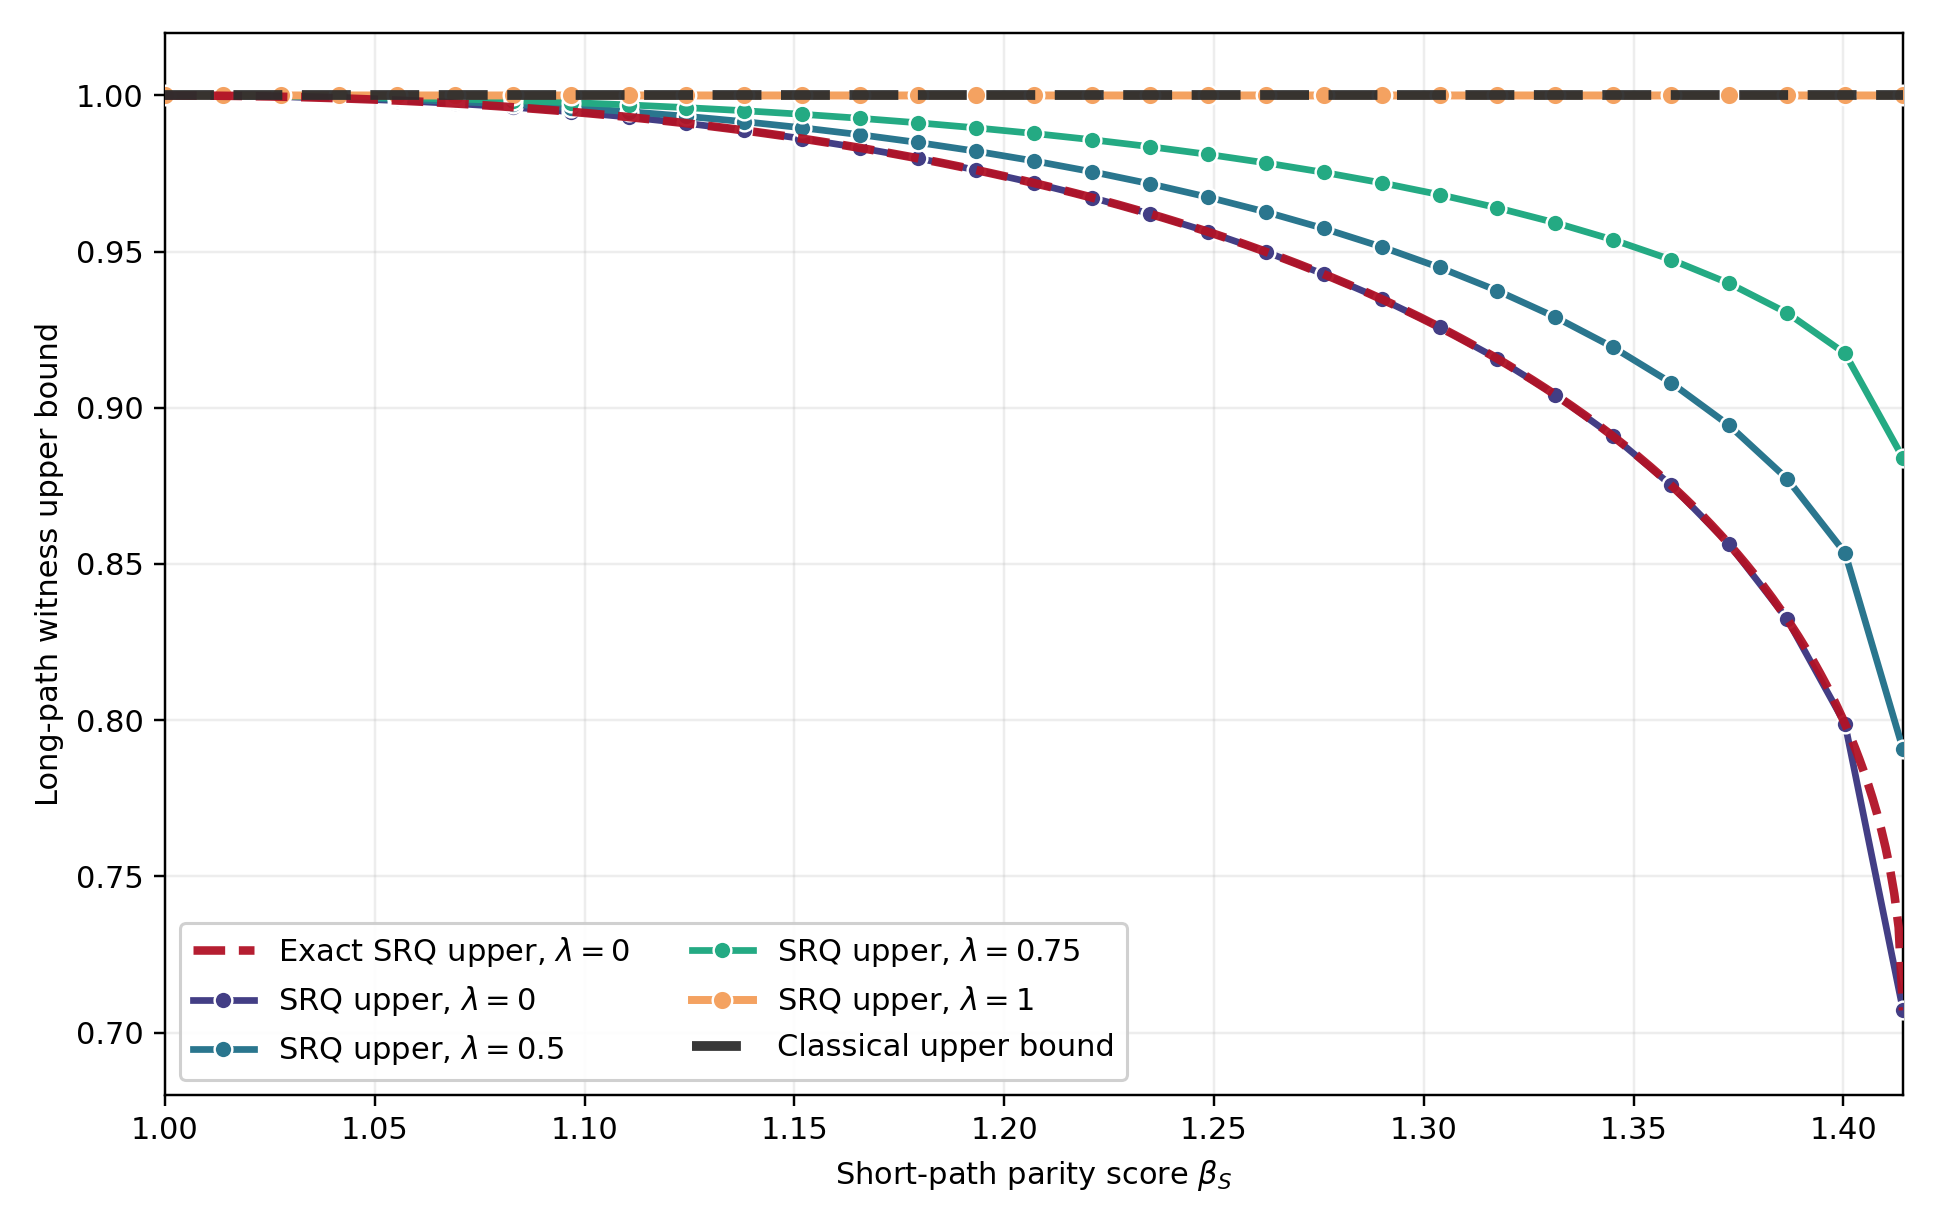
\includegraphics[width=0.8\linewidth]{tripartite_parity_tradeoff_vs_betaS.png}
 \caption{SRQ witness bound versus the nearby parity score. Markers and connecting lines give numerical SDP upper bounds at 31 scores for each \(\lambda\in\{0,0.5,0.75,1\}\); the red dashed curve is the analytical \(\lambda=0\) bound. The black dashed line is the isolated remote witness's local bound and the \(\lambda=1\) boundary. These binary-coarse-grained calculations illustrate Eq.~\eqref{eq:si-lambda-bound}, independently of the entropy certification.}
 \label{fig:si-srq-tradeoff}
\end{figure}
At maximal nearby score the SRQ bound is \(\sqrt{(1+\lambda^2)/2}\). The appropriate quantum comparison must obey the same nearby constraint: \(\beta_S=\sqrt2\) forces Alice's reflections to anticommute on the state support, giving
\begin{equation}
 P_{0,L},P_{1,L}\leq\frac1{\sqrt2},\qquad
 \overline W_L^{(\lambda)}\leq\frac{1+\lambda}{\sqrt2}.
 \label{eq:si-conditional-quantum}
\end{equation}
Indeed, \((A_0\pm A_1\overline C_{0L})^2=2\id\), and Bob's reflections commute with these operators. A GHZ state with \(A_0=Z,A_1=X,C_{0L}=X\) and \(B_{0L,1L}=(Z\pm X)/\sqrt2\) attains the bound along with the maximal nearby test. Quantum and SRQ boundaries coincide at \(\lambda=0\); their gap is positive for \(0<\lambda\leq1\). The unconditional remote quantum maximum \(\sqrt{1+\lambda^2}\) is not the comparison at fixed maximal nearby score.

\subsection{Why the scalar SRQ family misses this example}

At the main reference target, \(\nu=\eta_S=0.99\) and \(\eta_B=\eta_C=\eta=0.78\). The binary SRQ witness's additional identity terms vanish, so
\begin{equation}
 \overline\beta_L=\nu\eta\sqrt{1+\eta^2}<1,\qquad
 \beta_S=\nu\eta_S\sqrt{1+\eta_S^2}\in[1,\sqrt2],\quad\eta_S=0.99.
 \label{eq:si-reference-witness-values}
\end{equation}
Symmetry gives \(\overline W_L^{(\lambda)}=(1+\lambda)\overline\beta_L/2\), and hence
\begin{equation}
 \overline W_L^{(\lambda)}<\frac{1+\lambda}{2}
 \leq\sqrt{\frac{1+\lambda^2}{2}}\leq\Phi_\lambda(\beta_S),\qquad0\leq\lambda\leq1.
 \label{eq:no-scalar-srq-violation}
\end{equation}
The family therefore does not detect the reference behavior. The complete data nevertheless exclude SRQ, as the lifted Bell inequality in Appendix~\ref{app:remote-bell-witness} already shows, and their joint entropy bound certifies key. This illustrates a limitation of the selected witness family, not compatibility with SRQ or failure of all scalar witnesses.

\section{Joint phase information and erasure records}\label{app:ideal-mwrf}

For ternary outputs \((+1,-1,\perpout)\), define signed and detection coordinates \(V=(1,-1,0)\) and \(D=(1,1,0)\). They retain the full outcome information through \(P_\pm=(D\pm V)/2\), \(P_\perp=I-D\). In one common physical \(\rHybrid\) model, M contains the nearby behavior, all remote one- and two-party coordinates and the complete \(ZZZ\) key distribution. F contains the full nearby and remote behavior. W adds to M the three signed triples
\begin{equation}
 T_{1,0,0},\ T_{1,1,0},\ T_{1,3,0},\qquad
 T_{x,y,z}=\langle A_xV_{B,y}V_{C,z}\rangle,
\end{equation}
and R removes those three triples from F.

A computational-basis parent measurement applied only on the remote route removes GHZ coherence without changing M or R, including their ternary key probabilities. Eve retains its outcome and a purification labeling the GHZ/white-noise mixture; a computational-basis decomposition of the noise determines Alice's key bit as well. Her conditional entropy is therefore zero. The changed triples are precisely
\begin{equation}
 \Delta T_{1,0,0}=\nu\eta_B\eta_C\sin\theta_L,\quad
 \Delta T_{1,1,0}=-\nu\eta_B\eta_C\sin\theta_L,\quad
 \Delta T_{1,3,0}=\nu\eta_B\eta_C.
 \label{eq:coherent-differences}
\end{equation}
Thus W and F exclude this dephasing attack whenever these coherent correlations are nonzero; excluding that attack alone is not yet a quantitative entropy bound.

For \(\nu=\eta_S=1\), a stronger statement follows analytically. Let \(J\) denote both remote phase detectors clicking. Its probability \(\tau=\langle D_{B,3}D_{C,0}\rangle=\eta_B\eta_C\) is fixed already by M. W also fixes \(\langle A_1V_{B,3}V_{C,0}\rangle=\tau\), and hence
\begin{equation}
 P(J,A_1V_{B,3}V_{C,0}=-1)
 =\frac{P(J)-\langle A_1V_{B,3}V_{C,0}\rangle}{2}=0.
 \label{eq:si-ideal-phase-saturation}
\end{equation}
The phase parity determines Alice's bit on \(J\); the conditional entropy is at most one bit otherwise. Therefore \(H(A_1|B_3,C_0)\leq1-\tau\), and maximal nearby calibration gives \(H(A_0|E)\geq\tau\). The coherent-erasure attack matches F and attains \(\tau\). Consequently the smallest compatible secrecy entropy is exactly \(\eta_B\eta_C\) for W and F, while M and R admit zero secrecy. All four retain the same key distribution and reconciliation cost. Their ideal DW rates are thus
\begin{equation}
 K_{\mathrm W}=K_{\mathrm F}=\eta_B\eta_C+\min\{\eta_B,\eta_C\}-1,
 \qquad K_{\mathrm M}=K_{\mathrm R}=0.
 \label{eq:si-ideal-mwrf-rate}
\end{equation}
The W/F expression is understood as zero when nonpositive. Only M and the direct \(XXX\) triple were needed for the positive ideal bound. This is a sufficiency result, not a minimality claim or a requirement to retain each tilted triple.

\subsection{What the erasure flag contributes}\label{app:recording}

The flag distinguishes a missing observation from a genuine \(+1\). In the ideal symmetric target, assigning \(\perpout\mapsto+1\) gives \(P(B=-1|A=+1)=0\) and \(P(B=-1|A=-1)=\eta\), so the reconciliation cost is
\begin{equation}
 g_{\mathrm{bin}}(\eta)=\left(1-\frac\eta2\right)
 \hbin\!\left(\frac{1-\eta}{2-\eta}\right),
\end{equation}
instead of \(1-\eta\) with a ternary decoder record. This is a decoding benefit alone; no change to the secrecy estimate is needed.

A controlled comparison also isolates the benefit for phase estimation. At \(\nu=\eta_S=0.99\) and \(\eta_B=\eta_C=0.85\), two-point BFF bounds for the same hybrid settings do not certify key when the flag is merged in both test statistics and decoder records. Retaining it only for decoding, with the secrecy bound unchanged, gives \(K\geq0.0366\) bits per attempted key round. Resolving phase erasures as well gives \(K\geq0.1938\). The tilted observations remain binary-projected; the additional test information is the phase-erasure flag. Every comparison retains all attempted key rounds. These results separate gains in secrecy estimation from gains in decoding, rather than comparing different sources or measurements.

\section{Numerical entropy optimization}\label{app:bff}

\subsection{Observed statistics and the secrecy reduction}\label{app:composite-reduction}

The parties retain ternary remote records, but need not use every probability to lower-bound secrecy. We form composite Bob--Charlie observables while keeping Alice's key measurement unchanged. Every physical realization induces such a composite model with the same Alice--Eve state. Dropping unused observations and the separate-receiver structure therefore enlarges the admissible set and gives a conservative entropy bound. Reconciliation still uses each actual receiver's ternary key distribution:
\begin{equation}
 H(A_0|E)\geq H_{\mathrm{BFF}}(\mathcal C(\mathcal D)),\qquad
 K=H_{\mathrm{BFF}}(\mathcal C(\mathcal D))-\EC.
 \label{eq:si-composite-safety}
\end{equation}
Here \(\mathcal D=(P_S,P_L)\), and \(\mathcal C\) selects the observed composite statistics. The composite system is a secrecy relaxation, not a joint legitimate decoder.

The nearby binary effects and remote phase effects are
\begin{align}
 S_j^+&=B^S_{+|j}C^S_{+|0}+B^S_{+|1-j}C^S_{-|0},\quad j=0,1,\nonumber\\
 L_+&=B^L_{+|3}C^L_{+|0}+B^L_{-|3}C^L_{-|0},\nonumber\\
 L_-&=B^L_{+|3}C^L_{-|0}+B^L_{-|3}C^L_{+|0},\qquad
 L_\perp=\id-L_+-L_-.
\end{align}
Thus the phase statistic distinguishes the two double-click parities from a joint erasure. For the parity tests, write
\(\overline B_{+|j}=B^L_{+|j}+B^L_{\perpout|j}\),
\(\overline C_+=C^L_{+|0}+C^L_{\perpout|0}\) and
\(\overline C_-=C^L_{-|0}\). Their effective effects are
\begin{equation}
 R_j^+=\overline B_{+|j}\overline C_+
       +\overline B_{+|1-j}\overline C_-,
 \qquad j=0,1.
\end{equation}
The selected effect set is
\begin{equation}
 \mathcal O=
 \begin{cases}
 \{S_0^+,S_1^+,R_0^+,R_1^+\},&\rPCHSH,\\
 \{S_0^+,S_1^+,L_+,L_-\},&\rPhase,\\
 \{S_0^+,S_1^+,R_0^+,R_1^+,L_+,L_-\},&\rHybrid.
 \end{cases}
\end{equation}
For each \(O\in\mathcal O\), the constraints retain
\(\langle O\rangle\), \(\langle A_0^+O\rangle\) and
\(\langle A_1^+O\rangle\), together with Alice's marginals and normalization.
These define \(\mathcal W_{\mathrm{obs}}\) and its target values \(p_w\).
The matched long-only models omit the nearby effects \(S_j^+\).

\subsection{BFF optimization and operator constraints}\label{app:model-inventory}

At each interior right Gauss--Radau node \(t_i\), the BFF method~\cite{Brown2021,Brown2024} introduces one auxiliary \(Z_{a,i}\) for each binary key outcome and the polynomial
\begin{equation}
 {\cal B}_{t_i}=\sum_a\left[
 A_{a|0}\bigl(Z_{a,i}+Z_{a,i}^\dagger
 +(1-t_i)Z_{a,i}^\dagger Z_{a,i}\bigr)
 +t_iZ_{a,i}Z_{a,i}^\dagger\right].
 \label{eq:si-bff-polynomial}
\end{equation}
The final quadratic term is unconditional. Write \(A_x^+=A_{+|x}\), and let \(\mathcal O_L\) contain the remote members of \(\mathcal O\). The corresponding optimization is
\begin{equation}
 \begin{aligned}
 s_i(P)=\inf\;&\langle{\cal B}_{t_i}\rangle\\
 \text{subject to }\;&
 \langle w\rangle=p_w\quad(w\in\mathcal W_{\mathrm{obs}}),\\
 &A_x^+=(A_x^+)^\dagger=(A_x^+)^2,\qquad O=O^\dagger=O^2,\\
 &L_+L_-=0,\qquad L_++L_-+L_\perp=\id,\\
 &[A_x^+,O]=[A_x^+,Z_{a,i}]=[O_L,Z_{a,i}]=0,\\
 &\|Z_{a,i}\|\leq\alpha_i,\qquad
 \alpha_i\geq\tfrac32\max\{1/t_i,1/(1-t_i)\}.
 \end{aligned}
 \label{eq:si-bff-optimization}
\end{equation}
The infimum is over states and operators; constraints involving the phase effects are used only when those effects are included. Each binary effect has its complementary outcome. Projective measurements may be used after dilation.

Crucially, the nearby effects are not assumed to commute with Eve's auxiliaries or with the remote effects. The two routes concern alternative uses of the travelling systems, not independent measurements available simultaneously. The commuting remote effects in Eq.~\eqref{eq:si-bff-optimization} act separately from Eve; this distinction is retained in the moment relaxation.

For an \(m\)-point rule with endpoint \(t_m=1\), let
\(f_i=w_i/(t_i\ln2)\) and \(c_m=\sum_{i<m}f_i\).
Affine dual bounds \(\ell_i(P)\leq s_i(P)\) give
\begin{equation}
 H(A_0|E)\geq H_{\mathrm{BFF}}(P)
 :=\max\left\{0,c_m+\sum_{i<m}f_i\ell_i(P)\right\}.
 \label{eq:si-bff-bridge}
\end{equation}
The endpoint is bounded analytically, so only the interior nodes require optimization. Separate optimization of those nodes preserves the lower-bound direction.

\subsection{Relaxation and numerical settings}

We use a level-two noncommutative moment relaxation~\cite{NPA2007,NPA2008,Pironio2010}. Its degree-two basis contains at most one auxiliary letter and is enriched by \(A_x^+O_LZ_a\) and \(A_x^+O_LZ_a^\dagger\). The moment matrix obeys \(\Gamma\succeq0\). Norm-localizing matrices use the identity and single physical projectors and obey \(\Gamma(g_{a,1})\succeq0\), \(\Gamma(g_{a,2})\succeq0\), for \(g_{a,1}=\alpha_i^2\id-Z_{a,i}^\dagger Z_{a,i}\) and \(g_{a,2}=\alpha_i^2\id-Z_{a,i}Z_{a,i}^\dagger\). These rules specify the relaxation without imposing extra cross-route commutations.

The plotted curves use \(m=4\), with auxiliary bounds \((17,4,8)\); the erasure-record control uses \(m=2\) and bound \(5\). Curve searches use MOSEK with relative-gap, primal-feasibility and dual-feasibility tolerances \(10^{-7}\). These stopping tolerances are not entropy error bars. The reported entropy inequalities include conservative deductions for positivity residuals and quadrature-node evaluation before the reconciliation cost is subtracted.

At the reference target \(\nu=\eta_S=0.99\), \(\eta_B=\eta_C=0.78\), a four-point nearby--phase bound gives
\begin{equation}
 H(A_0|E)\geq0.3327199,\qquad
 \EC\leq0.2554235,\qquad
 K>0.07729.
 \label{eq:si-reference-rate}
\end{equation}
It uses no remote parity-test observations and therefore applies to both phase and hybrid protocols. Together with Appendix~\ref{app:attack}, it establishes the same-target security separation.

An affine entropy inequality remains valid at other targets with the same algebra and observed coordinates. The curves take the strongest available node bounds and combine them through Eq.~\eqref{eq:si-bff-bridge}; they do not interpolate optimized entropy values. Hybrid models may inherit bounds from either subprotocol, and routed models may inherit long-only bounds. The first positive grid point is a sufficient efficiency, and coincident curves may use the same inequality without having equal optimal rates. Lower quadrature orders also give positive bounds at the reference point, but these finite-order checks do not establish convergence of the moment hierarchy.

\section{Remote insecurity at the nonideal reference point}\label{app:attack}

\subsection{A physical attack consistent with the complete distant data}

Take \(\nu_0=0.99\), \(\eta_B=\eta_C=\eta_0=0.78\) and \(\theta_0=\arctan\eta_0\). Let \(P_L^{\mathrm{ref}}\) be the hybrid target and \(Q_{\mathrm{GHZ}}\) the ideal lossless GHZ behavior at the same settings. A compatible attack mixes this quantum behavior with deterministic local response tables:
\begin{equation}
 P_L^{\mathrm{ref}}=qQ_{\mathrm{GHZ}}+\sum_\lambda w_\lambda D_\lambda,\qquad
 q,w_\lambda\geq0,\qquad q+\sum_\lambda w_\lambda=1.
 \label{eq:si-exact-attack}
\end{equation}
Here \(D_\lambda\) assigns an output to every input of each party, including the receivers' erasures. Choosing the weights is a finite linear feasibility problem: Eq.~\eqref{eq:si-exact-attack} is imposed on every conditional probability, not merely on the Bell scores. A nonnegative decomposition exists with \(q\simeq0.1620\) and local weight \(\gamma=1-q>0.8380\). Its deterministic part is balanced in Alice's key outcomes,
\begin{equation}
 \sum_\lambda w_\lambda D_\lambda^A(a|0)=\frac{\gamma}{2},
 \qquad a=\pm1.
\end{equation}
Thus the local label reveals Alice's bit on a fraction \(\gamma\) of rounds independently of its value. Every component is a physical realization; the construction is not an outer relaxation of the quantum set.

Eve retains the component label and the predetermined local responses. She marks her record as erased in the GHZ component. On each known bit she produces a simulated click with probability \(\eta_0/\gamma\), flips the bit with probability \(\epsilon=(1-\nu_0)/2\), and otherwise reports \(\perpout\). This is possible because \(\gamma>\eta_0\). For either required receiver \(R\),
\begin{equation}
 \begin{aligned}
 P(\widetilde R=a|A=a)&=\eta_0(1-\epsilon),\\
 P(\widetilde R=-a|A=a)&=\eta_0\epsilon,\\
 P(\widetilde R=\perpout|A=a)&=1-\eta_0.
 \end{aligned}
\end{equation}
These are precisely the target ternary key channels. Lemma~\ref{lem:si-simulation} excludes a positive remote-only key guarantee in the stated Alice-only class, including her preprocessing. The attack matches all distant observations but need not match the nearby branch. The positive bound in Eq.~\eqref{eq:si-reference-rate} applies when those nearby observations are included.

\subsection{The distant behavior is nevertheless Bell-nonlocal}\label{app:remote-bell-witness}

For this witness only, assign Bob's erasure to \(+1\) and define the unnormalized expression
\begin{align}
 S_{C+}=\sum_{a,b=\pm1}ab\bigl[&P(a,b,+|0,0,0)+P(a,b,+|1,0,0)\nonumber\\
 &+P(a,b,+|0,1,0)-P(a,b,+|1,1,0)\bigr].
\end{align}
Every fully local model obeys
\begin{equation}
 S_{C+}\leq2P(C_0=+).
 \label{eq:si-lifted-chsh}
\end{equation}
Indeed, conditioning a deterministic local table on Charlie's fixed-input outcome \(+\) leaves a local Alice--Bob CHSH response with bound two. Averaging over those tables gives the unnormalized inequality directly, without a fair-sampling assumption.

For the target, \(P(C_0=+)=\eta_0/2\), and the ratio is
\begin{equation}
 \frac{S_{C+}}{2P(C_0=+)}
 =\nu_0\eta_0(\cos\theta_0+\sin\theta_0)
 =\frac{\nu_0\eta_0(1+\eta_0)}{\sqrt{1+\eta_0^2}}
 \simeq1.0838>1.
\end{equation}
The complete distant behavior is therefore Bell-nonlocal despite allowing the attack above. This witness uses test probabilities, not selection of the retained key data, and does not certify genuine tripartite nonlocality.

\bibliographystyle{apsrev4-2}
\bibliography{references}

\end{document}
